\apendice{Documentación técnica de programación}

\section{Introducción}

Esta sección pretende aclarar todos los conceptos relativos a las cuestiones técnicas y de programación llevadas a cabo en el presente Trabajo de Fin de Máster.

\section{Estructura de directorios}
Este apartado presenta la estructura de los directorios y carpetas usados en el proyecto. Esta estructura es la siguiente:

\begin{itemize}
	\item \textbf{web:} esta carpeta almacena todos los recursos web, desde las páginas jsp hasta los ficheros css pasando por los ficheros javascript o las imágenes usadas.
	\begin{itemize}
		\item \textbf{css:} carpeta con los ficheros css que dan estilo a la plataforma web.
		\item \textbf{jquery\textbackslash bootstrap:} ficheros pertenecientes al framework Bootstrap.
		\item \textbf{jquery\textbackslash fileupload:} ficheros que permiten la subida de ficheros al servidor.
		\item \textbf{jquery\textbackslash rutassemanticas:} ficheros javascript para el manejo de las páginas que componen la plataforma web de Rutas Semánticas.
		\item \textbf{jquery\textbackslash rutassemanticas\textbackslash threads:} estos ficheros permiten consultar los estados de los hilos que pueden ser ejecutados.
		\item \textbf{jquery\textbackslash steps:} los ficheros ubicados bajo la carpeta \textit{steps} permiten el manejo de los sistemas de información del estado de ejecución de los procesos.
		\item \textbf{images:} carpeta con imágenes y/o logos.
		\item \textbf{pages:} páginas JSP del sistema web.
	\end{itemize}
	\item \textbf{src:} la carpeta con todas las clases Java queda dividida en:
	\begin{itemize}
		\item \textbf{controller\textbackslash algorithm:} ficheros pertenecientes a la ejecución del algoritmo.
		\item \textbf{controller\textbackslash connection:} estas clases permiten establecer la conexión contra la Base de Datos.
		\item \textbf{controller\textbackslash servlet:} clases de servidor.
		\item \textbf{model\textbackslash dao:} estas clases pertenecen al DAO (Data Access Object) y permiten realizar operaciones CRUD sobre el sistema.
		\item \textbf{model\textbackslash data:} estas clases forman el modelo de la plataforma web.
	\end{itemize}
\end{itemize}

\section{Manual del programador}

La presente sección indica cómo instalar las herramientas necesarias para el correcto desempeño de todo el sistema.

Si se opta por una máquina virtual, primero se deberá contar con el software Virtual Box instalado en el sistema anfitrión.

\subsection{Virtual Box}
El software de virtualización seleccionado ha sido Oracle VM Virtual Box en su versión 5.1. Este programa ha sido instalado sobre Windows 10, sistema que actúa como anfitrión.

La descarga de este software se puede realizar desde la siguiente dirección web: \url{https://www.virtualbox.org/wiki/Downloads}. En el caso de que el sistema anfitrión sea diferente, se deberá optar por la descarga correspondiente.

\subsection{Ubuntu 16.04 LTS}
Como servidor se ha optado por la versión 16.04 de Ubuntu en su versión de escritorio. El sistema ha sido instalado sobre una máquina virtual haciendo uso del software mencionado en la sección anterior.

Para descargar una imagen de este Sistema Operativo se ha de acceder al siguiente enlace: \url{https://www.ubuntu.com/download/desktop}

El nombre de usuario y contraseña son los siguientes:

\begin{itemize}
	\item Usuario: \textbf{rs}.
	\item Contraseña: \textbf{rs}.
\end{itemize}

A partir de este momento se indican los pasos necesarios para una instalación de todo el software restante sobre la distribución 16.04 LTS.

\subsubsection{Recursos del sistema}

El sistema ha contado con los siguientes recursos hardware durante la fase de desarrollo y pruebas:

\begin{itemize}
	\item Espacio en disco: 80 GiB en disco de estado sólido.
	\item CPU: 4 cores con disposición del 100\% de su capacidad.
	\item Memoria RAM: 8 GiB de RAM.
	\item Memoria de Vídeo dedicada: 128 MiB.
	\item Red: conectividad de red por NAT.
\end{itemize}


\subsection{PostgreSQL 9.6, PgAdmin 3 y PostGIS}
PostgreSQL puede ser instalado en Ubuntu desde la consola de comandos. Para ello se han de seguir unos sencillos pasos.

\subsubsection{PostgreSQL}

La configuración aquí mostrada puede verse en el tutorial mostrado en la página wiki de PostGIS \cite{installpost:info}.

El primer paso es añadir el repositorio al fichero sources.list:

\begin{lstlisting}[language=bash]
  sudo sh -c 'echo "deb http://apt.postgresql.org/pub/repos/apt xenial-pgdg main" >> /etc/apt/sources.list'
\end{lstlisting}

El siguiente paso consiste en añadir las claves y actualizar los repositorios de Ubuntu:

\begin{lstlisting}[language=bash]
	wget --quiet -O - http://apt.postgresql.org/pub/repos/apt/ACCC4CF8.asc | sudo apt-key add -
	sudo apt-get update
\end{lstlisting}

Ahora se puede comenzar la instalación de Postgres mediante la siguiente línea en la consola de comandos:
\begin{lstlisting}[language=bash]
	sudo apt-get install postgresql-9.6 postgresql-server-dev-9.6
\end{lstlisting}

Si se desea hacer uso de PgAdmin 3, se podrá instalar mediante el siguiente comando:
\begin{lstlisting}[language=bash]
	apt-get install pgadmin3
\end{lstlisting}

\subsubsection{PostGIS}

Una vez que Postgres ha sido instalado, se ha de instalar la extensión PostGIS mediante los siguientes comandos de consola:

\begin{lstlisting}[language=bash]
	sudo apt-get install postgresql-9.6-postgis-2.3 postgresql-contrib-9.6
\end{lstlisting}
Una vez termina, se ha de continuar con este comando:

\begin{lstlisting}[language=bash]
	sudo apt-get install postgis
\end{lstlisting}

Se puede obtener más información en la página web oficial de PostGIS: \url{http://www.postgis.net/}.

\subsubsection{pg\_cron}

\quotes{pg\_cron} \cite{pgcron:info} es un programador de tareas para PostgreSQL basado en cron. Este programador permitirá realizar tareas de mantenimiento sobre la Base de Datos en los tiempos marcados al programar las tareas.

Para usar este complemento de chrome primero se ha de instalar y configurar, a continuación, se mencionan los pasos necesarios.


El primer paso consistirá clonar el repositorio mediante el siguiente comando:

\begin{lstlisting}[language=bash]
	git clone https://github.com/citusdata/pg_cron.git
\end{lstlisting}

Después se debe acceder a la carpeta y exportar la ruta de la siguiente forma:

\begin{lstlisting}[language=bash]
	cd pg_cron
	export PATH=/usr/pgsql-9.6/bin:$PATH
\end{lstlisting}

El último comando a ejecutar es el siguiente:

\begin{lstlisting}[language=bash]
	make && sudo PATH=$PATH make install
\end{lstlisting}

Ahora se debe abrir el fichero \textit{postgresql.conf} situado en \textit{/etc/postgresql/9.6/main}. En este fichero se ha de indicar la Base de Datos sobre la que actuará pg\_cron. Las dos últimas líneas del fichero han de lucir de la siguiente forma:
\begin{lstlisting}[language=bash]
	shared_preload_libraries = 'pg_cron'
	cron.database_name = 'rutassemanticas'
\end{lstlisting}

Par que los cambios funcionen se ha de reiniciar el servicio:
\begin{lstlisting}[language=bash]
	sudo service postgresql restart
\end{lstlisting}

\subsubsection{Configuración básica de PostgreSQL}

Una vez instalados esta serie de paquetes, se puede continuar con la configuración de PostgreSQL antes de cerrar la consola de comandos. El siguiente paso consistirá en asignar una contraseña al usuario  \quotes{postgres} como se detalla a continuación.

El primer paso es acceder a PostgreSQL mediante:
\begin{lstlisting}[language=bash]
	sudo -u postgres psql postgres
\end{lstlisting}
Este comando nos introducirá en la consola del SGBD, para asignar una nueva contraseña se ha de indicar el siguiente comando:

\begin{lstlisting}[language=bash]
	\password postgres
\end{lstlisting}

En este caso, se ha decidido asignar la clave \quotes{postgres} para recordarla de forma sencilla.

Como recomendación no se debe instalar PostGIS sobre la Base de Datos por defecto (postgres), para seguir esta recomendación, se creará una nueva Base de Datos a la que se asignarán el resto de extensiones y tablas:

\begin{lstlisting}[language=bash]
	CREATE DATABASE rutassemanticas;
	\connect rutassemanticas;
\end{lstlisting}

Es el momento de añadir alguna extensión adicional a esta Base de Datos:

\begin{lstlisting}[language=bash]
	CREATE EXTENSION adminpack;
	CREATE EXTENSION postgis;
	CREATE EXTENSION fuzzystrmatch;
	CREATE EXTENSION postgis_sfcgal;
	CREATE EXTENSION pg_cron;
\end{lstlisting}

Estas extensiones permitirán manejar las consultas lanzadas sobre PostGIS y habilitar cron.

Ahora se debe salir del gestor mediante el comando:
\begin{lstlisting}[language=bash]
	\q
\end{lstlisting}

A partir de este momento se puede conectar contra el host local desde PgAdmin 3. Para ello se ha de indicar los siguientes parámetros:

\begin{itemize}
	\item Nombre: se debe teclear \textbf{localhost}.
	\item Host: como en el caso anterior, será \textbf{localhost}.
	\item Username: usaremos el nombre de usuario \textbf{postgres}.
	\item Password: y su contraseña asignada hace unos instantes \textbf{postgres}.
\end{itemize}

En la Figura \ref{conexion} se pueden visualizar estos valores.

\begin{figure}[h]
  \centering
    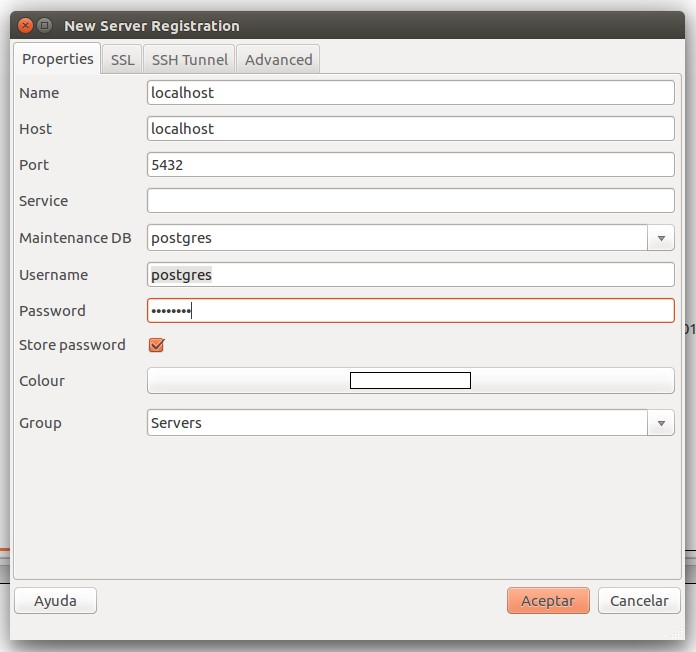
\includegraphics[width=0.6\textwidth]{../img/instalacion/conexion.jpg}
  \caption{Conexión contra el host local.}
  \label{conexion}
\end{figure}

Una vez conseguida la conexión contra el sistema, se procederá a crear un nuevo usuario y se añadirán nuevas extensiones. De esta forma se comprueba que tanto PostgreSQL, como PostGIS funcionan de forma correcta para su futuro uso.

Para crear un nuevo usuario se ha de clicar sobre la sección \quotes{Login Roles} del host local. El asistente solicita distintos parámetros como se observa en las Figuras \ref{nr1}, \ref{nr2} y \ref{nr3}:

\begin{itemize}
	\item Nombre de usuario: \textbf{rs}.
	\item Password: \textbf{rs}.
	\item Privilegios: super usuario, creación de bases de datos y creación de roles.
\end{itemize}

\begin{figure}[h]
  \centering
    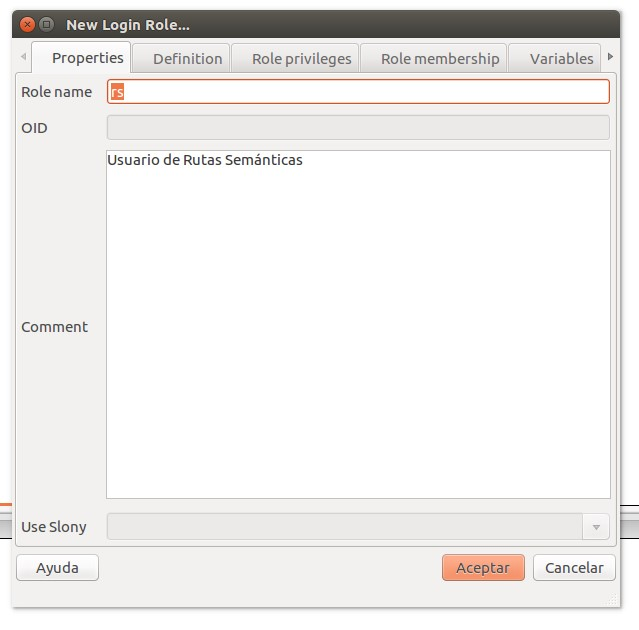
\includegraphics[width=0.6\textwidth]{../img/instalacion/nr1.jpg}
  \caption{Nombre de usuario.}
  \label{nr1}
\end{figure}

\begin{figure}[h]
  \centering
    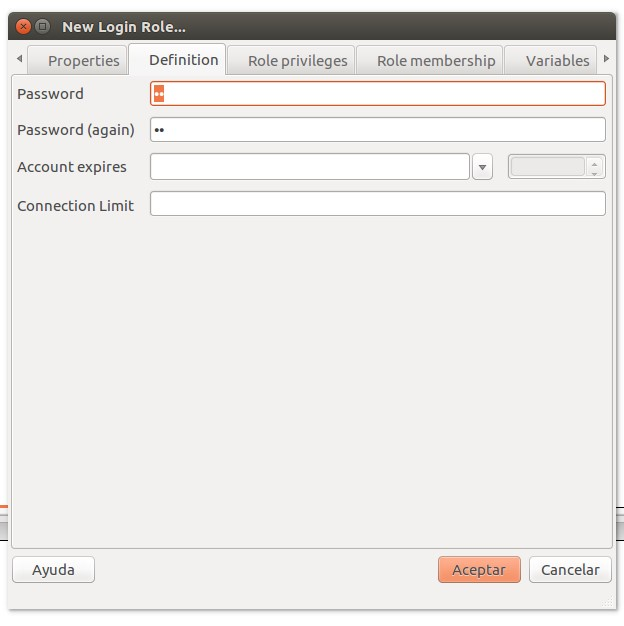
\includegraphics[width=0.6\textwidth]{../img/instalacion/nr2.jpg}
  \caption{Contraseña.}
  \label{nr2}
\end{figure}

\begin{figure}[h]
  \centering
    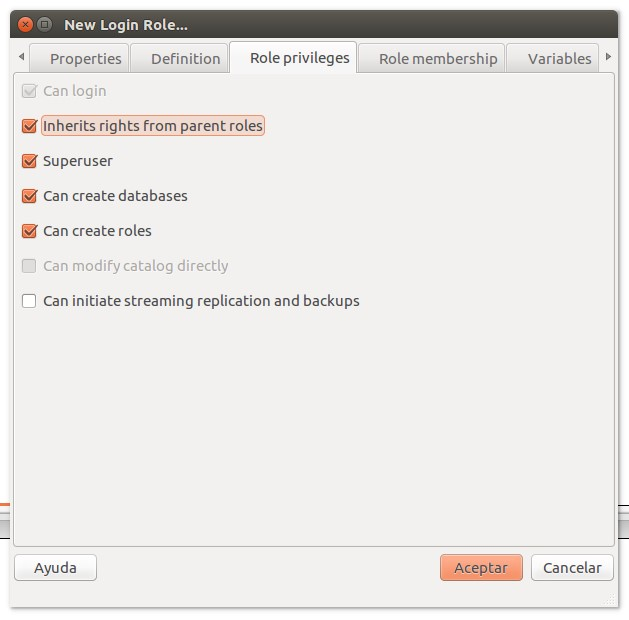
\includegraphics[width=0.6\textwidth]{../img/instalacion/nr3.jpg}
  \caption{Privilegios.}
  \label{nr3}
\end{figure}

Una vez se cuenta con un nuevo usuario, se podrá asignar la Base de Datos creada por consola al usuario creado. Para ello se clica con botón derecho sobre la Base de Datos y se modifica el valor de propietario como se aprecia en la Figura \ref{asignacion}.

\begin{figure}[h]
  \centering
    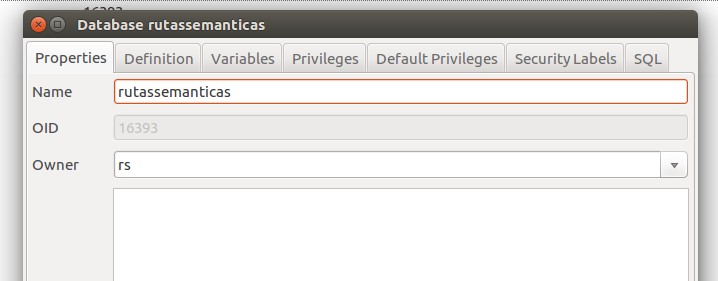
\includegraphics[width=0.6\textwidth]{../img/instalacion/asignacion.jpg}
  \caption{Asignacion de usuario rs a rutassemanticas.}
  \label{asignacion}
\end{figure}

\subsubsection{Tareas programadas con pg\_cron}
Para crear tareas programadas con pg\_cron se han de ejecutar sentencias select contra cron.schedule.

Estas son las tres tareas que se han programado en el SGBD:

\begin{lstlisting}[language=bash]
	SELECT cron.schedule('55 23 * * *', 'VACUUM');
	SELECT cron.schedule('59 23 * * *', $$DELETE FROM tfm_ruta WHERE es_temporal = true$$);
		SELECT cron.schedule('59 23 * * *', $$DELETE FROM tfm_experimento WHERE es_temporal = true$$);
\end{lstlisting}

Estas tareas permiten realizar operaciones de mantenimiento (como VACCUM) y borrado de rutas y pruebas temporales.

En este punto se cuenta con un SGBD instalado en el sistema, un usuario con una Base de Datos asignada y las extensiones necesarias. En los siguientes apartados se muestra cómo instalar el resto de componentes.

\subsection{Java y Glassfish 4}
A continuación, se mostrará cómo instalar Java y el servidor Glassfish sobre Ubuntu \cite{installjava:info}. Para ello, se han de seguir los siguientes pasos:

La lista de comandos es la siguiente:
\begin{lstlisting}[language=bash]
	sudo apt-get install python-software-properties
	sudo add-apt-repository ppa:webupd8team/java
	sudo apt-get update
	sudo apt-get install oracle-java8-installer
\end{lstlisting}

Si ahora se teclea en la consola:
\begin{lstlisting}[language=bash]
	java -version
\end{lstlisting}

Se observará que Java ya se encuentra instalado en el sistema en su versión más reciente.  Es recomendable asignar la variable JAVA\_HOME de la siguiente forma:

\begin{lstlisting}[language=bash]
	export JAVA_HOME=/usr/lib/jvm/java-8-oracle
\end{lstlisting}


A continuación se mostrará cómo instalar Glassfish en su versión 4.1.1, para ello, es necesario descargar todos sus ficheros mediante el siguiente comando:


\begin{lstlisting}[language=bash]
	wget http://download.java.net/glassfish/4.1.1/release/glassfish-4.1.1.zip
\end{lstlisting}

Una vez finalizada la descarga, es posible desempaquetar Glassfish sobre la carpeta /opt del sistema y se cambiará su pertenencia al usuario rs:

\begin{lstlisting}[language=bash]
	sudo mv glassfish-4.1.1.zip /opt
	unzip glassfish-4.1.1.zip
	sudo rm glassfish-4.1.1.zip
	sudo chown -R rs:rs /opt 
\end{lstlisting}

Para comprobar que Glassfish funciona, se levantará el servidor situándose en la carpeta /opt y tecleando el siguiente comando:
\begin{lstlisting}[language=bash]
	glassfish4/bin/asadmin start-domain
\end{lstlisting}

Si todo sucede de forma correcta, el \quotes{domain1} quedará levantado y corriendo. Antes de finalizar se ha de configurar la memoria asignada a la JVM en la consola de administración del servidor.

\subsubsection{Configuración de Glassfish}
Para acceder a la consola mencionada anteriormente, se ha de abrir un navegador y teclear \quotes{localhost:4848} que es el puerto de escucha de configuración de Glassfish. En unos segundos, la consola quedará a disposición del usuario.

Se ha de acceder a la sección \quotes{Configurations} -> \quotes{Server config} -> \quotes{JVM} y asignar el valor 2048m a la variable Xmx del listado. Esta configuración se puede apreciar en la Figura \ref{glassconfig}.

\begin{figure}[h]
  \centering
    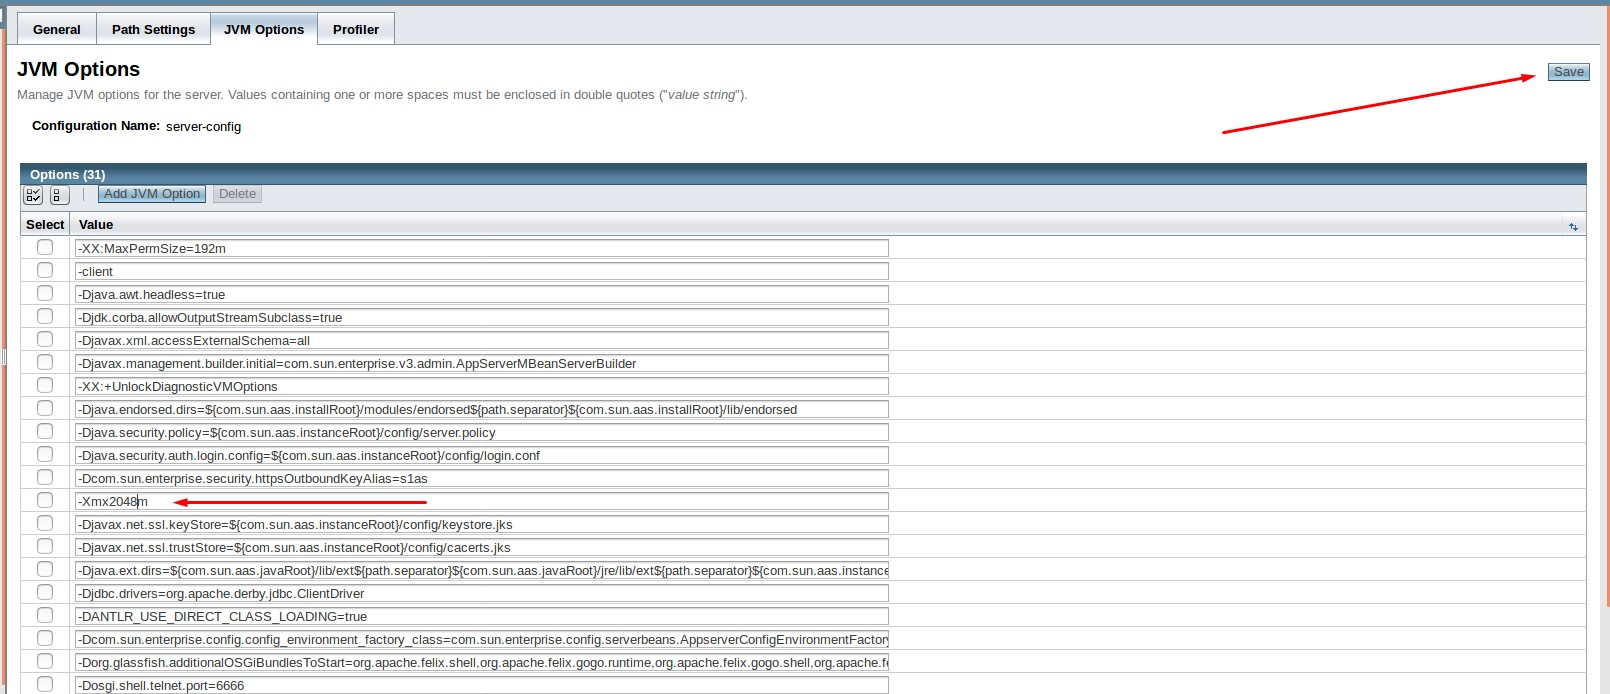
\includegraphics[width=0.6\textwidth]{../img/instalacion/glassconfig.jpg}
  \caption{Configuración de memoria de Glassfish.}
  \label{glassconfig}
\end{figure}

\subsection{NetBeans}
Como IDE se ha usado NetBeans, para instalar este entorno se ha de acceder al sección de descargas de su desarrollador y elegir la versión que cuente con Java EE por defecto (Figura \ref{descnet}.

\begin{figure}[h]
  \centering
    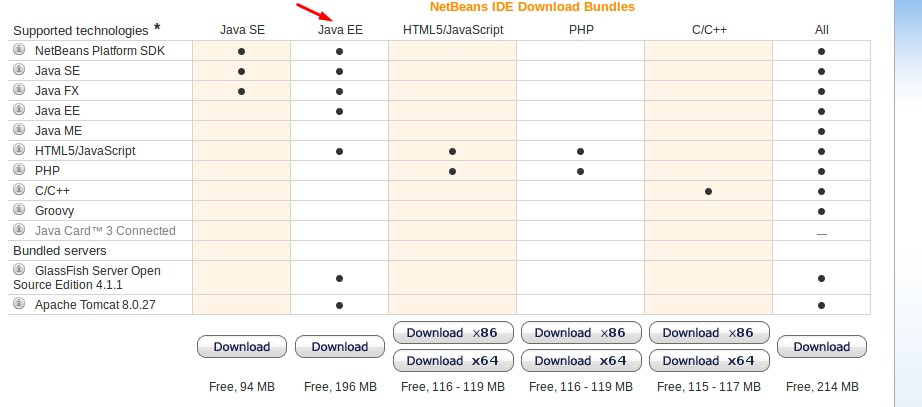
\includegraphics[width=0.6\textwidth]{../img/instalacion/descnet.jpg}
  \caption{Descarga de NetBeans.}
  \label{descnet}
\end{figure}

El IDE cuenta con un sencillo instalador que guía al usuario en todos los pasos necesarios. Como ya se cuenta con Glassfish en el sistema, se desmarcará la opción que permite una nueva instalación de este servidor. Al finalizar, el IDE se lanzará y se podrá comenzar a trabajar. Si por alguna razón no encuentra la ruta adecuada al JDK instalado, en el apartado siguiente se comenta cómo solucionar este pequeño inconveniente. Además, se muestra cómo ligar a NetBeans con Glasssfish.

\subsubsection{Configuración}
En el caso de que NetBeans no localice el JDK, se ha de abrir el fichero \quotes{netbeans.conf} de la carpeta \textbackslash etc, situada dentro de la carpeta del IDE. La línea que ha de modificarse es la siguiente:

\begin{lstlisting}[language=bash]
	netbeans_jdkhome="/usr/lib/jvm/java-8-oracle"
\end{lstlisting}

Para indicar el servidor a NetBeans se ha de acceder a la ventana de configuración de servidores del IDE, localizada en: \quotes{Tools} -> \quotes{Servers}. En este momento se mostrará una ventana que permitirá seleccionar el servidor que se desea instalar además de otros parámetros. Todo el proceso de configuración queda descrito en las siguientes figuras:  \ref{sv1}, \ref{sv2} y \ref{sv3}, información obtenida de \cite{servnet:info}.

\begin{figure}[h]
  \centering
    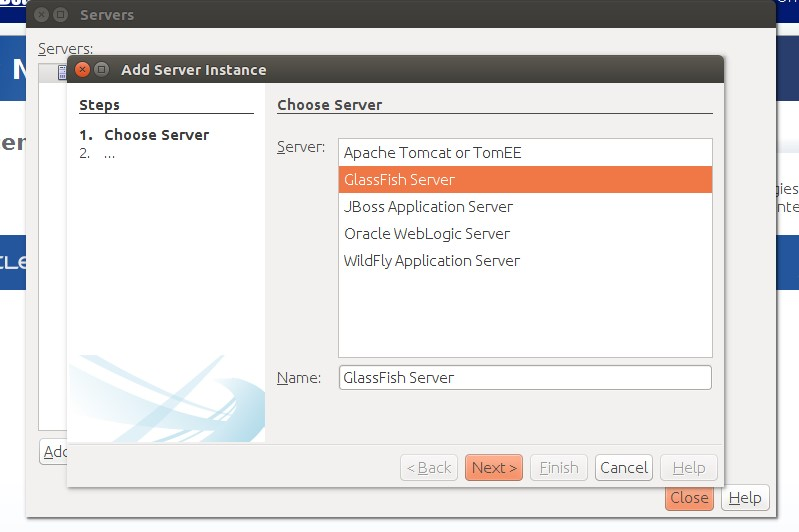
\includegraphics[width=0.6\textwidth]{../img/instalacion/sv1.jpg}
  \caption{Selección de servidor.}
  \label{sv1}
\end{figure}

\begin{figure}[h]
  \centering
    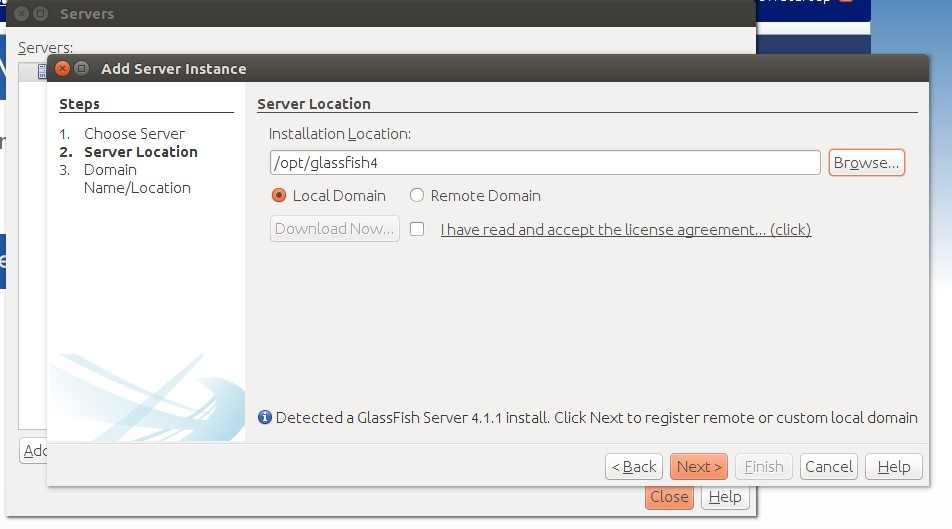
\includegraphics[width=0.6\textwidth]{../img/instalacion/sv2.jpg}
  \caption{Localización del servidor en el sistema.}
  \label{sv2}
\end{figure}

\begin{figure}[h]
  \centering
    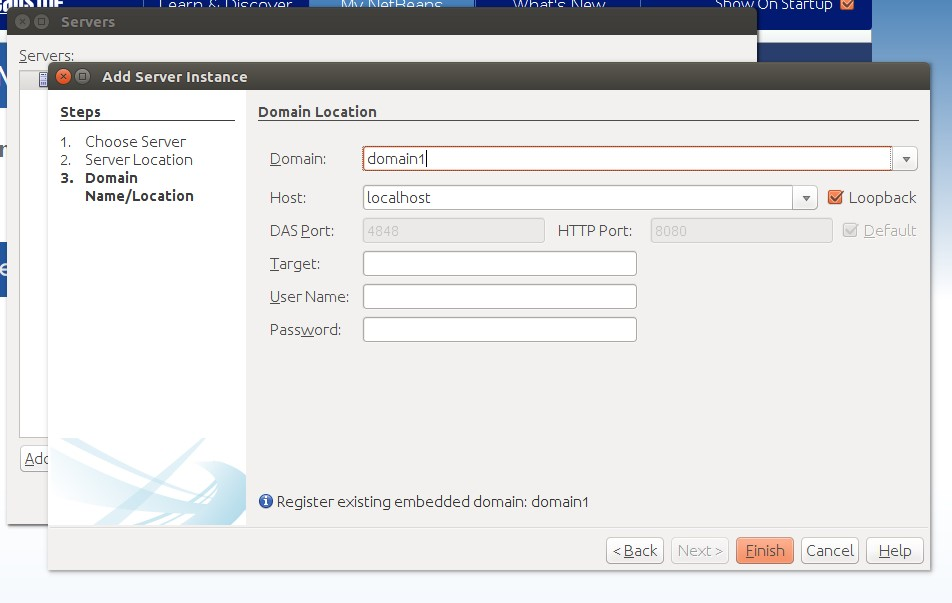
\includegraphics[width=0.6\textwidth]{../img/instalacion/sv3.jpg}
  \caption{Indicación del dominio.}
  \label{sv3}
\end{figure}

\subsection{QGIS}

Durante el desarrollo de este trabajo se ha hecho uso de las capacidades de QGIS para visualizar resultados y rutas sobre mapas OpenStreetMap. QGIS se encuentra incluido en el repositorio de Ubuntu y solo es necesario teclear el siguiente comando en la consola:

\begin{lstlisting}[language=bash]
	sudo apt-get install qgis
\end{lstlisting}

\subsection{Herramientas de OpenStreetMap}
Para instalar las herramientas pertenecientes a OpenStreetMap que permiten procesar ficheros de tipo osm se han de seguir los pasos mostrados a continuación.

\subsubsection{Osmosis}
La instalación de Osmosis se realiza de la siguiente forma:
\begin{lstlisting}[language=bash]
	sudo apt-get install osmosis
\end{lstlisting}

\subsubsection{Osmfilter y Osmconvert}
Estas dos herramientas se encuentran dentro de las utilidades del siguiente paquete:
\begin{lstlisting}[language=bash]
	sudo apt-get install osmctools
\end{lstlisting}

\section{Compilación, instalación y ejecución del proyecto}

El proyecto ha sido creado y desarrollado bajo el IDE NetBeans, por tanto, se mostrará cómo ejecutar el mismo desde este IDE. Además, se mostrará cómo desplegar la plataforma web sobre el propio servidor Glassfish.

\section{Recuperación de la Base de Datos}
Para recuperar la Base de Datos sobre PostgreSQL se usará la interfaz ofrecida por PgAdmin3. Los pasos son sencillos y mostrados en las figuras \ref{uno}, \ref{dos}, \ref{tres}, \ref{cuatro}, \ref{cinco} y \ref{seis}.

\begin{figure}[h]
  \centering
    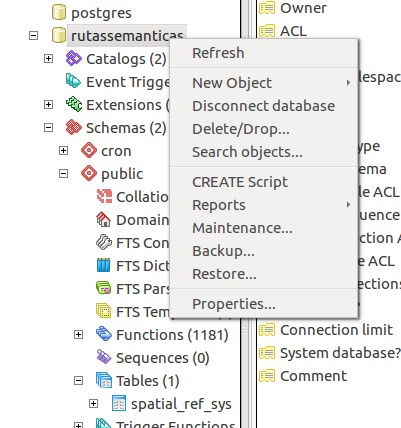
\includegraphics[width=0.6\textwidth]{../img/restoredb/uno.jpg}
  \caption{Click sobre \quotes{Restore}.}
  \label{uno}
\end{figure}

\begin{figure}[h]
  \centering
    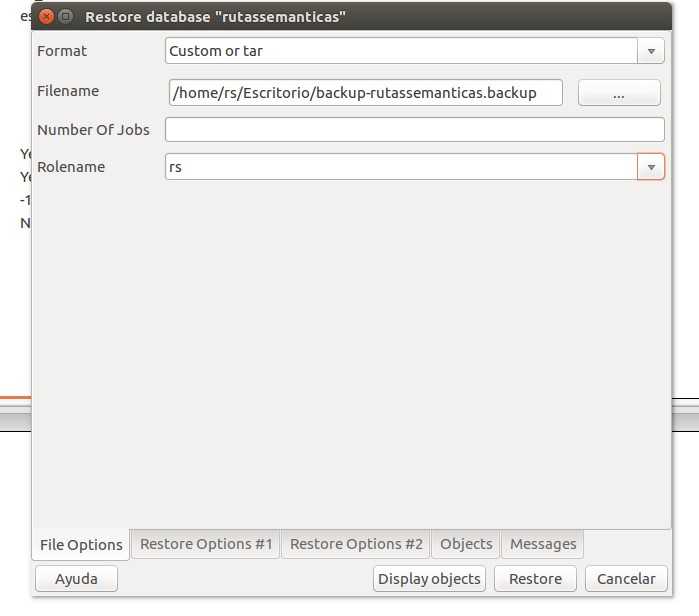
\includegraphics[width=0.6\textwidth]{../img/restoredb/dos.jpg}
  \caption{Selección del fichero de backup.}
  \label{dos}
\end{figure}

\begin{figure}[h]
  \centering
    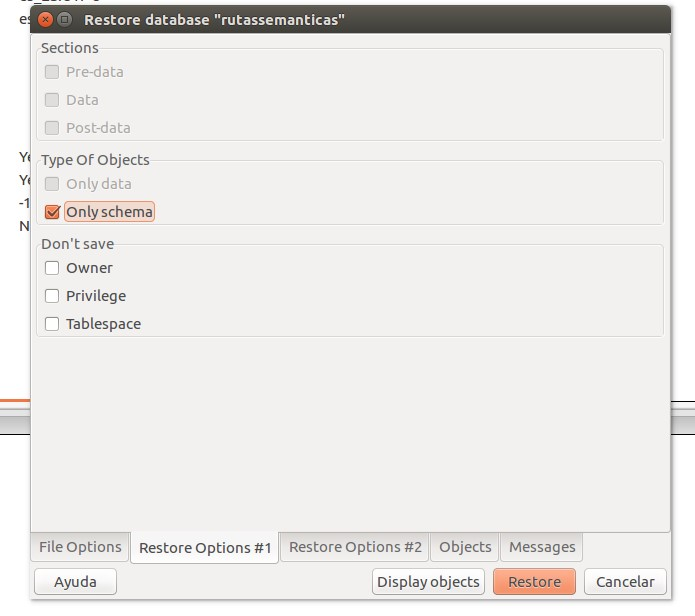
\includegraphics[width=0.6\textwidth]{../img/restoredb/tres.jpg}
  \caption{Selección de opciones.}
  \label{tres}
\end{figure}

\begin{figure}[h]
  \centering
    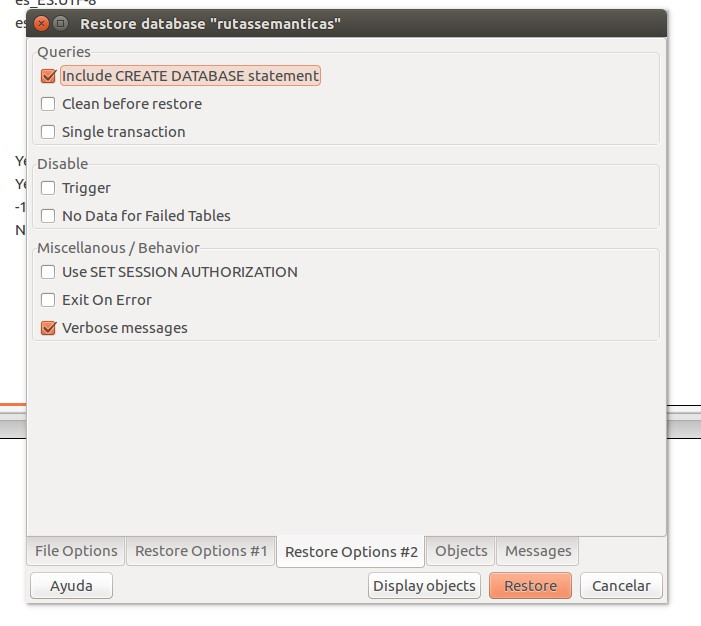
\includegraphics[width=0.6\textwidth]{../img/restoredb/cuatro.jpg}
  \caption{Opciones adicionales.}
  \label{cuatro}
\end{figure}

\begin{figure}[h]
  \centering
    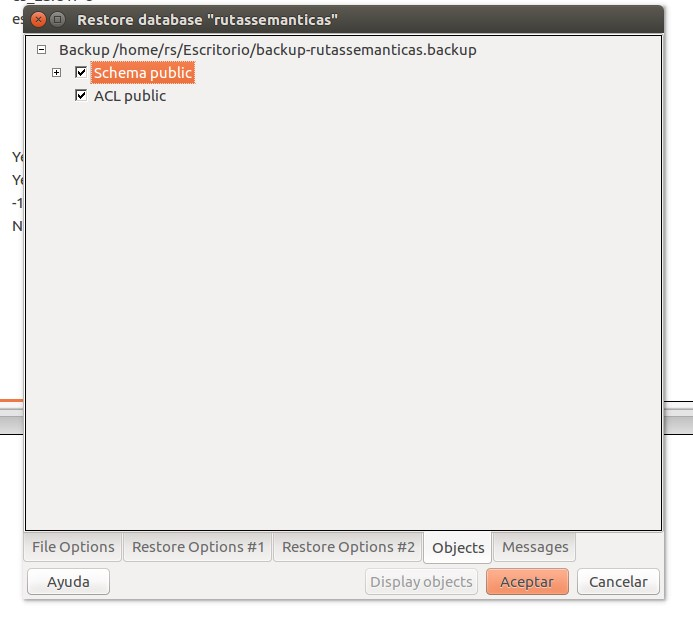
\includegraphics[width=0.6\textwidth]{../img/restoredb/cinco.jpg}
  \caption{Tablas a restaurar.}
  \label{cinco}
\end{figure}

\begin{figure}[h]
  \centering
    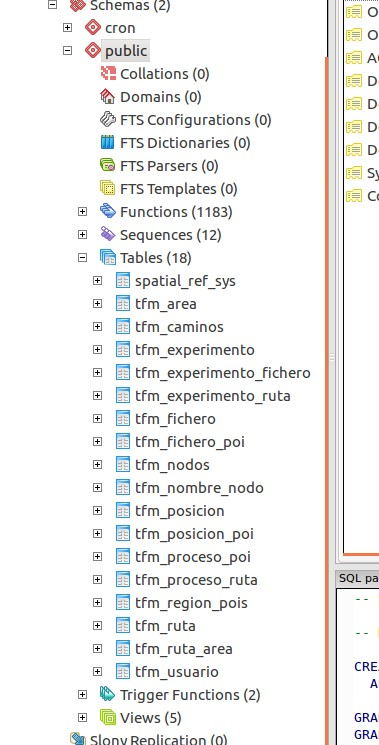
\includegraphics[width=0.6\textwidth]{../img/restoredb/seis.jpg}
  \caption{Resultado obtenido.}
  \label{seis}
\end{figure}


Una vez restaurada, es posible lanzar la plataforma web mediante alguna de las opciones mostradas a continuación.

\subsection{Área por defecto}
Si se desea contar con un área por defecto, se puede crear con la siguiente sentencia SQL. A esta área pertenecerán las rutas a las que no se pueda o quiera asignar una área concreta.
\textbf{
	insert into tfm\_area (nombre, descripcion, min\_lat, min\_long, max\_lat, max\_long, activa, fecha\_creacion) values('Desconocida', 'Área con rutas desconocidas', -90, -180, 90, 180, true, now());
}

\subsection{NetBeans}

La ejecución o despliegue desde NetBeans es tan simple como clicar con el botón derecho sobre el proyecto y elegir la opción \quotes{run}. La Figura \ref{netbeansrun} muestra esta opción.

\begin{figure}[h]
  \centering
    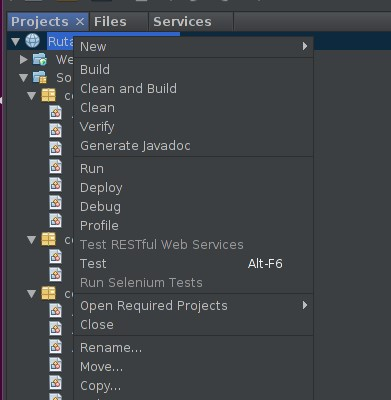
\includegraphics[width=0.6\textwidth]{../img/glass/netbeansrun.jpg}
  \caption{Despliegue desde NetBeans.}
  \label{netbeansrun}
\end{figure}

El servidor será lanzado por NetBeans así que no se han de seguir pasos adicionales.

\subsection{Despliegue de la plataforma web}
Para poder acceder a la plataforma web, primero se ha de obtener un fichero de extensión \textbf{war} desde el IDE y después desplegarlo mediante los comandos de Glassfish.

Para obtener este fichero simplemente se ha de construir el proyecto y acceder a la carpeta \quotes{dist} del mismo. En esta carpeta se encontrará el fichero war que se ha de desplegar en el servidor.

Para no perder este fichero en una posible desinstalación de NetNBeans se creará una carpeta llamada \textit{Proyectos} en la que se copiará este fichero.

Una vez copiado se han de seguir estos pasos \cite{auto:info}:

\begin{enumerate}
	\item Acceder a la carpeta \textit{glassfish4} dentro de /opt.
	\item Lanzar el dominio mediante estos comandos:
	\begin{lstlisting}[language=bash]
		bin/asadmin
		start-domain domain1		
	\end{lstlisting}
	\item Lanzar el comando de ejecución de despliegue:
	\begin{lstlisting}[language=bash]
		bin/asadmin deploy /home/rs/Proyectos/RutasSemanticas.war
	\end{lstlisting}
\end{enumerate}

La Figura \ref{deploy} muestra el resultado de la ejecución.
\begin{figure}[h]
  \centering
    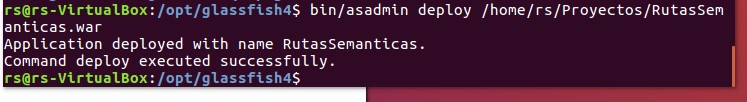
\includegraphics[width=0.6\textwidth]{../img/glass/despliegue.jpg}
  \caption{Despliegue en Glassfish.}
  \label{deploy}
\end{figure}

Si se desea cancelar el despliegue simplemente se deberá ejecutar el siguiente comando:

\begin{lstlisting}[language=bash]
	bin/asadmin undeploy /home/rs/Proyectos/RutasSemanticas
\end{lstlisting}

El resultado es mostrado en la Figura \ref{undeploy}.

\begin{figure}[h]
  \centering
    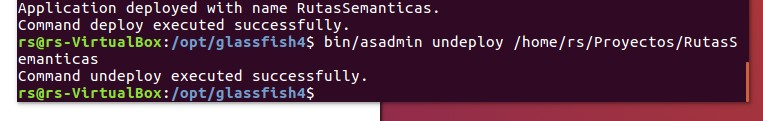
\includegraphics[width=0.6\textwidth]{../img/glass/undeploy.jpg}
  \caption{Cancelación del despliegue.}
  \label{undeploy}
\end{figure}

Si se desea detener el dominio se deberán seguir los mismos pasos que para iniciarlo. El comando ha de ser el siguiente:

\begin{lstlisting}[language=bash]
	bin/asadmin
	stop-domain domain1		
\end{lstlisting}